\FloatBarrier
\section{构筑参数与收益稳定性}\label{sec:construction}
\subsection{交换性决定一次均值与二次方差}
固定$N=24$、$a=b=d=1$、$c=2$、$n=10$、$h=4$，
令普通非攻击牌数为$s$，普通攻击牌数为$t=19-s$，$0\le s\le19$。
必需组件数量保持不变，故$p=25/253$，而收益阶段可消耗牌的数量随$s$变化。

\begin{proposition}\label{prop:polynomial}
在上述固定规模替换下，条件收益均值与方差分别为
\begin{align}
\mu(s)&=\frac{64}{35}+\frac{264}{175}s,\label{eq:linear-mean}\\
\sigma^2(s)&=\frac{13824}{1225}
+\frac{1064832}{116375}s-\frac{282624}{581875}s^2.\label{eq:quadratic-variance}
\end{align}
条件方差在合法整数$s=9$时最大。
\end{proposition}

\begin{proof}
把A、B与两张C之外的20张实体牌暂视作普通实体。
启动事件$I=1$不区分这些实体的D、T、S标签。
记$Z$为收益阶段C的数量，$H_i$为第$i$张普通实体牌处于收益阶段的指示变量。
在其中固定选$s$张标记为S后，有
$X_s=Z+\sum_{i=1}^sH_i$。
成功时至少一张C已在前缀，故$Z\in\{0,1\}$。
下述期望均以$I=1$为条件。交换性保证
\[
z:=\E Z,\quad \alpha:=\E H_i,\quad
\beta:=\E(H_iH_j)\ (i\ne j),\quad
\gamma:=\E(ZH_i)
\]
与实体标签无关。
令$\phi(v,k)$表示总数为$v$、A/B各一张、C有$k$张的牌组，
前10张满足三类组件要求的概率；它由式\eqref{eq:singleton}给出。
一张指定实体进入收益阶段的概率为$4/24$，
两张指定实体共同进入的概率为$4\cdot3/(24\cdot23)$。
先指定收益实体，再在剩余牌中计算前缀事件，得到
\begin{equation}\label{eq:tagged-moments}
\begin{aligned}
z&=\frac{2(4/24)\phi(23,1)}p=\frac8{35},&
\alpha&=\frac{(4/24)\phi(23,2)}p=\frac{33}{175},\\
\beta&=\frac{[12/(24\cdot23)]\phi(22,2)}p=\frac{93}{3325},&
\gamma&=\frac{2[12/(24\cdot23)]\phi(22,1)}p=\frac6{175}.
\end{aligned}
\end{equation}
于是
\begin{equation}\label{eq:indicator-second}
\E X_s=z+s\alpha,\qquad
\E X_s^2=z+s\alpha+s(s-1)\beta+2s\gamma.
\end{equation}
将它们代入$\mu=8\E X_s$、
$\sigma^2=64[\E X_s^2-(\E X_s)^2]$，即得式
\eqref{eq:linear-mean}、\eqref{eq:quadratic-variance}。
方差二次项为$64(\beta-\alpha^2)<0$，
其连续顶点为$s_*=13865/1472\approx9.419158$。
最近的合法整数为9，故整数最大值在$s=9$取得。
\end{proof}

由上述矩表达式可见，条件均值由一阶矩确定，方差进一步取决于二阶矩及协方差项。
随着$s$增加，可消耗数量的均值上升；中等比例下两种牌类混合最明显，
接近两端时可消耗性更易确定，条件方差因而先升后降。
式\eqref{eq:tagged-moments}刻画了启动条件引起的牌组组成偏移。

\begin{figure}[htbp]
\centering
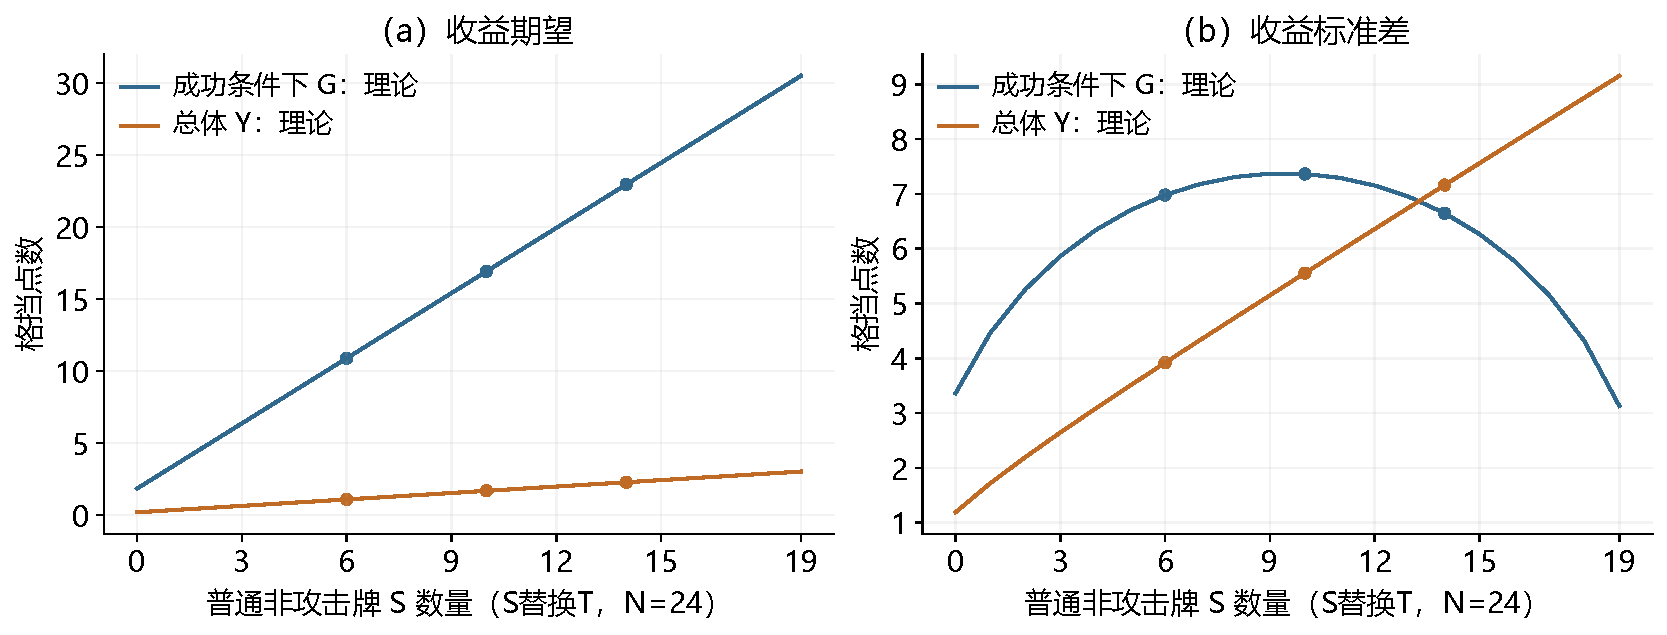
\includegraphics[width=\linewidth]{05_mean_and_sd.pdf}
\caption{固定$N$的S/T替换下，条件与总体收益的精确期望和标准差。
标记点对应$s=6,10,14$；右图显示方差指标与均值指标具有不同变化规律。}\label{fig:mean-sd}
\end{figure}

\begin{table}[htbp]
\centering\small
\caption{固定规模替换的代表性精确结果，三组均有$p=25/253$}\label{tab:baseline}
\begin{tabular}{rrrrrr}
\toprule
$s$ & $t$ & $\mu$ & $\sigma$ & $\mathbb E(Y)$ & $\operatorname{SD}(Y)$ \\
\midrule
6 & 13 & 10.8800 & 6.9785 & 1.0751 & 3.9183 \\
10 & 9 & 16.9143 & 7.3630 & 1.6714 & 5.5528 \\
14 & 5 & 22.9486 & 6.6472 & 2.2676 & 7.1598 \\
\bottomrule
\end{tabular}

\end{table}

图\ref{fig:mean-sd}和表\ref{tab:baseline}显示，条件标准差从$s=10$到14下降，
总体标准差却继续上升。不同层次的收益变量，具有不同的方差变化规律。
此外，在同一个实体排列中把一张T改标为S，$I$不变而$X$逐样本不减，
因此条件收益和总体收益均关于$s$一阶随机占优。
因此均值和正阈值尾概率随$s$非减，方差则遵循式\eqref{eq:quadratic-variance}的二次关系。

\subsection{全期望、全方差与零值混合}
在$I=0$时$Y=0$，在$I=1$时$Y=G$。
因此$\E(Y\mid I)=I\mu$、$\V(Y\mid I)=I\sigma^2$。
依次对$I$取期望与方差，得到
\begin{equation}\label{eq:total-moments}
\E(Y)=p\mu,\qquad
\V(Y)=
\underbrace{p\sigma^2}_{\text{成功后的条件波动}}
+\underbrace{p(1-p)\mu^2}_{\text{成功/失败条件均值差异}}.
\end{equation}
基准结果为
\begin{equation}\label{eq:total-values}
\E(Y)=\frac{2960}{1771}\approx\BaseMean,\qquad
\V(Y)\approx\BaseWithin+\BaseActivation=\BaseVar.
\end{equation}
两个方差贡献分别占17.3741\%与82.6259\%。
其中第二项体现成功与失败两类条件均值之间的差异。

\begin{figure}[htbp]
\centering
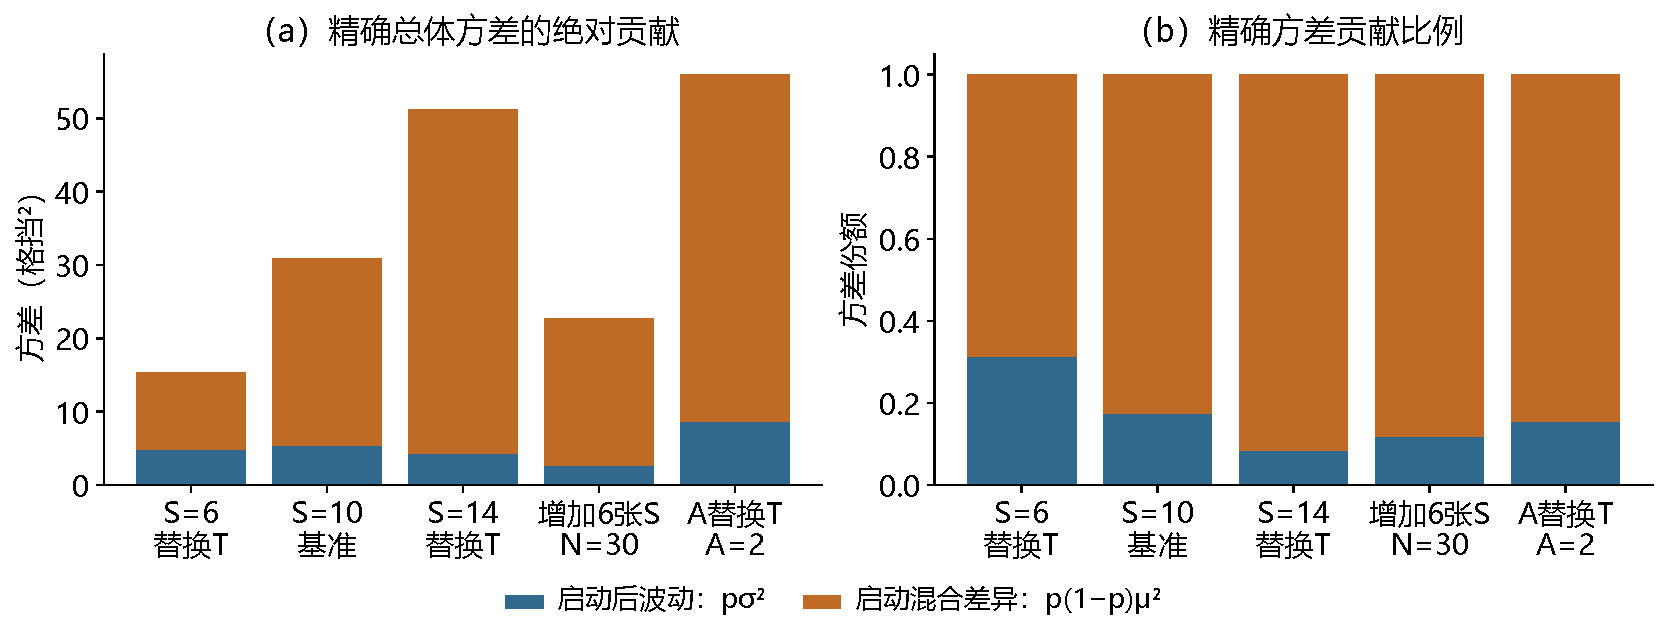
\includegraphics[width=\linewidth]{06_variance_decomposition.pdf}
\caption{不同操作下总体方差的精确分解。左图为绝对贡献，右图为份额；
基准中成功/失败条件均值差异占82.63\%。}\label{fig:variance}
\end{figure}

图\ref{fig:variance}显示，总体方差由条件波动和成功概率共同决定。
固定$p$时，均值$\mu$上升还会放大$p(1-p)\mu^2$，
从而解释图\ref{fig:mean-sd}中条件与总体标准差的不同走向。
当$\mu>0$时，记$\CV(U)=\SD(U)/\E(U)$，由式\eqref{eq:total-moments}还有
\begin{equation}\label{eq:cv}
\CV(Y)^2=\frac{\CV(G\mid I=1)^2+1-p}{p}.
\end{equation}
较小的$p$本身就会提高相对波动。
因此总体标准差、零收益概率与总体均值应联合解读。

\subsection{增删与替换操作的不同权衡}
表\ref{tab:operations}均以基准为参照，固定$n=10,h=4$。
增加或删除牌张改变$N$；替换保持$N$不变。
多副本A按第\ref{sec:model}节的协议激活一张，其余未揭示副本仍可被C消耗。

\begin{table}[htbp]
\centering\small
\caption{明确操作成本后的代表性构筑指标，均为精确理论值}\label{tab:operations}
\setlength{\tabcolsep}{5pt}
\begin{tabular}{lrrrrrr}
\toprule
相对基准操作 & $N$ & $p$ & $\mu$ & $\mathbb E(Y)$ & $\operatorname{SD}(Y)$ & $\mathrm{CV}(Y)$ \\
\midrule
基准 & 24 & 0.0988 & 16.9143 & 1.6714 & 5.5528 & 3.3223 \\
删除6张S & 18 & 0.2255 & 11.1304 & 2.5098 & 5.6406 & 2.2474 \\
增加6张S & 30 & 0.0515 & 20.2160 & 1.0401 & 4.7599 & 4.5763 \\
以A替换1张T & 24 & 0.1640 & 18.5640 & 3.0451 & 7.4803 & 2.4565 \\
以C替换1张T & 24 & 0.1245 & 18.5435 & 2.3088 & 6.6399 & 2.8760 \\
以C替换1张S & 24 & 0.1245 & 17.0483 & 2.1226 & 6.1989 & 2.9204 \\
\bottomrule
\end{tabular}

\end{table}

直接增加6张S，条件均值从16.9143提高到20.2160，
但启动概率从0.0988降到0.0515，总体均值从1.6714降到1.0401。
与固定$N$的S/T替换相比，这一操作额外引入了组件稀释。
图\ref{fig:tradeoff}展示了条件收益与组件可及性的权衡：
在所研究的S增删序列中，增加S提高条件回报，却降低固定预算内的组件齐全概率。

\begin{figure}[htbp]
\centering
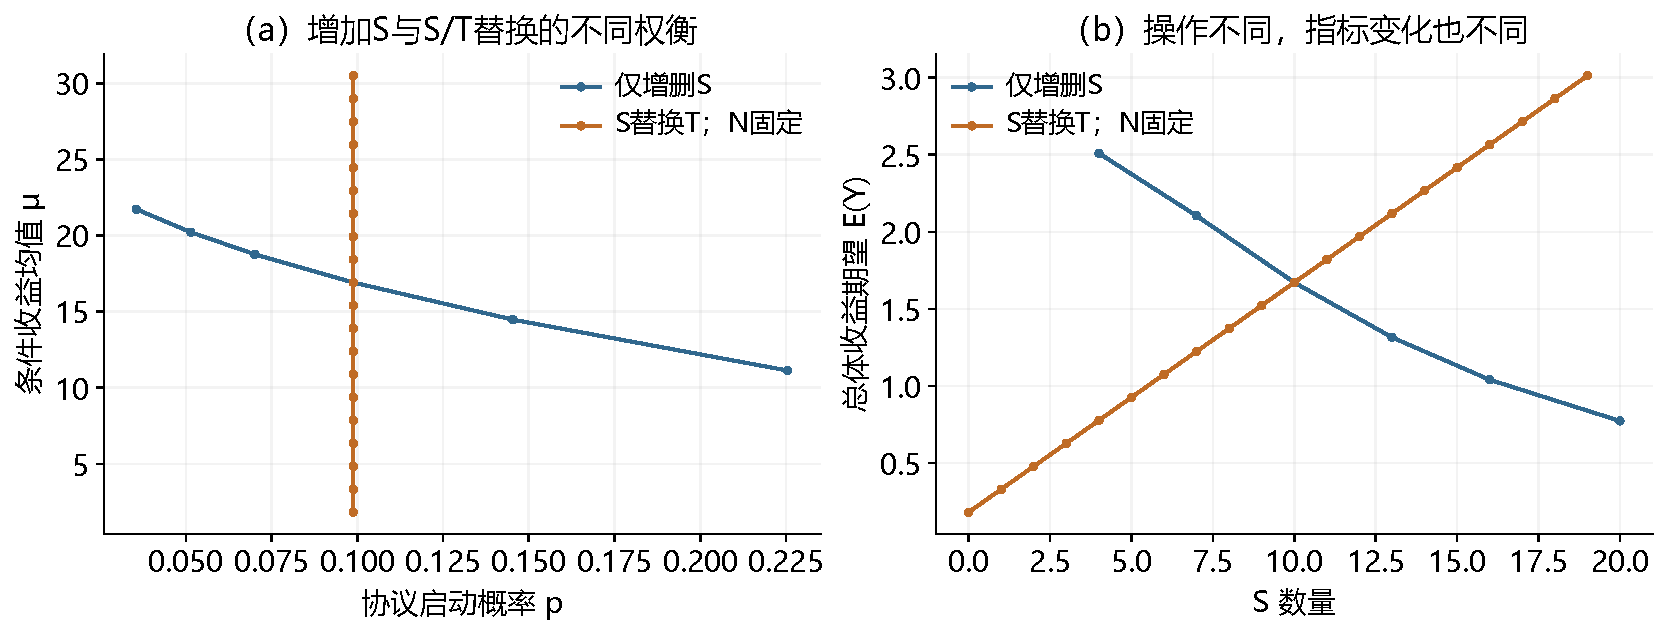
\includegraphics[width=\linewidth]{10_construction_tradeoffs.pdf}
\caption{增加S与固定规模S/T替换的不同效果，曲线均为精确理论值。
左图比较启动概率与条件均值，右图比较总体均值。}\label{fig:tradeoff}
\end{figure}

直接增加6张S后，总体标准差虽从5.5528降至4.7599，
零收益概率却从90.4490\%升至94.9149\%，$\CV(Y)$从3.3223升至4.5763。
总体标准差下降的同时，零收益更加频繁，故应结合均值、零收益率与变异系数解读。
固定$N$做S/T替换时，成功概率恒定，条件与总体格挡均值同向上升。
攻击牌T的输出价值可以在进一步的攻防联合模型中考察。

复制关键牌则同时改变可及性与剩余非攻击比例。
以C替换T或S具有相同的启动概率，却有不同的条件均值，
因为两种来源使非攻击牌总数的变化不同。
因此，相同总牌数下，不同类别的构成依然产生不同的收益分布；
构筑比较应具体说明增删或替换的牌类与数量。
